\subsection*{AI 1. \textit{Numeración}}

Las páginas serán enumeradas a partir del Índice de Contenidos, con números romanos colocados en la parte media inferior de cada página. A partir de la Introducción, todas las páginas serán enumeradas con números arábigos ubicados en la parte inferior derecha. No usar la palabra “página” antes de la numeración de las páginas.

\subsection*{AI 2. \textit{Palabras Clave (tamaño 10)}}

Debajo del resumen deberán indicarse hasta cinco (5) palabras clave, también conocidas como descriptores. En la sección del resumen en inglés (abstract) deberán también incluirse las palabras clave (keywords). Se colocarán inmediatamente debajo del resumen (abstract) con la indicación en negrita Palabras Clave (Keywords) y a continuación en la misma línea las palabras. 

\subsection*{AI 3. \textit{Títulos y Subtítulos}}

El título de los capítulos debe numerarse con número arábigo consecutivos, y ser escrito con letra mayúscula y en negrita en tamaño 16 puntos escritos a partir del margen izquierdo en una nueva página. El subtítulo (o si corresponde, el inicio de un texto), comenzará 1 espacio más abajo. El subtítulo será precedido por un número arábigo y se escribirá con letra mayúscula en negrita y tamaño 14 puntos, escrito a partir del margen izquierdo. El subtítulo del 3er. orden (o si corresponde un texto), comenzará 1 espacio más abajo. Los subtítulos de 3er. orden podrán ser idénticos al anterior, pero escritos con letra minúscula (la primera con mayúscula), sin negritas, y el texto comenzará una línea más abajo. Si a continuación del subtítulo de 3er. orden se escribe un subtítulo de 4º orden deberá dejarse un espacio. Los subtítulos de 4º, 5º u orden superior, serán idénticos al de 3er orden y el texto comenzará en la misma línea.

Las palabras y/o frases no deben ser abreviadas en títulos y resumen la primera vez que aparecen. 

\subsection*{AI 4. \textit{Figuras, Tablas, Ecuaciones y Notas al pie (tamaño 10)}}

Las Figuras, Ilustraciones (Estilo Figura) y Tablas deben ser colocadas en secuencia en el texto, y siempre que sea posible próximas de donde son indicadas. Las figuras deben ser de buena calidad (en una impresión deberían notarse todos los detalles que fueran importantes) y llevar una leyenda concisa en su parte inferior. Todas las ilustraciones y figuras deben ser numeradas (Ej “Figura \ref{fig:Tiempo de reverberacion}” etc.) nunca excediendo los márgenes de impresión. En caso de incorporarse a la sección de anexo, la numeración debe estar antepuesta por la letra A y reestablecer la misma a 1 (ej ''Figura \ref{fig:Comparativa R}”).

Las letras en los dibujos o gráficos no deberían ser menores a 1,5 mm de alto. Si es posible, las letras en todas las ilustraciones deben ser del mismo tamaño, y usar el idioma castellano (no inglés). Se recomienda no utilizar solamente colores para identificar características de un gráfico (en caso de mediciones, utilizar símbolos diferentes con cada color, así además se pueden identificar por la forma). Las leyendas de las Tablas (Ej “Tabla 1”) deben ser posicionadas centradas encima de las mismas (Estilo Título Figuras). Tanto para las Figuras como para las Tablas, junto a la identificación debe suministrarse una pequeña descripción explicativa del contenido. En caso de incorporarse a la sección de anexo, la numeración debe estar antepuesta por la letra A y reestablecer la misma a 1 (ej “Tabla \ref{Tab:1}”).

Si la Figura o Tabla es una copia sacada de una de las fuentes bibliográficas, es preferible vectorizar mediante algún programa de dibujo para mejorar la resolución. También debe constar en el título la fuente mediante el número de referencia bibliográfica.
Las ecuaciones y expresiones matemáticas deben estar centradas y numeradas en secuencia, con el número de la ecuación justificado a la derecha y entre paréntesis, utilizando numeración arábiga.
En caso de utilizar notas al pie deben estar referidas con algún símbolo en superíndice (Ej texto†) en el cuerpo del texto y en el pie de la misma página referir el comentario en letra tamaño 10 interlineado simple. Se sugiere que la nota al pie no supere los tres renglones.

Las ecuaciones y expresiones matemáticas deben estar centradas y numeradas en secuencia, con el número de la ecuación a la derecha y entre paréntesis, utilizando numeración arábiga. En ecuaciones de varias líneas, la numeración debe ser ubicada en la última línea. Las fórmulas y el texto deben ser separados por una línea. Las ecuaciones deben ser hechas en la misma fuente del texto, con los índices 3 puntos abajo. Deben usarse símbolos convencionales y unidades SI. Las ecuaciones deben ser citadas en el texto (''Ecuación \eqref{eq: LF}", etc.).

En el texto debe definirse cada símbolo, con sus unidades, y representadas en formato itálica (''donde S es la superficie del elemento en $m^2$, TR es el tiempo de reverberación del recinto a una cierta frecuencia expresado en segundos y $\alpha$ es el coeficiente de absorción sonora, adimensional”).

\begin{equation}
    \label{eq: LF}
    \tau_{d} = \frac{\int_{0}^{\theta_{lim}} \tau \sin \sin \theta \cos \cos \theta \ \dd \theta}{\int_{0}^{\theta_{lim}} \sin \sin \theta \cos \cos \theta \ \dd \theta}
\end{equation}

Para ingresar ecuaciones y se enumeren automáticamente, pueden usar el formato de la ecuación anterior (es una tabla de 1 fila y dos columnas, la primera celda está el editor de ecuaciones y en la segunda celda el número de ecuación): 


    \begin{figure}[h]
        \centering
        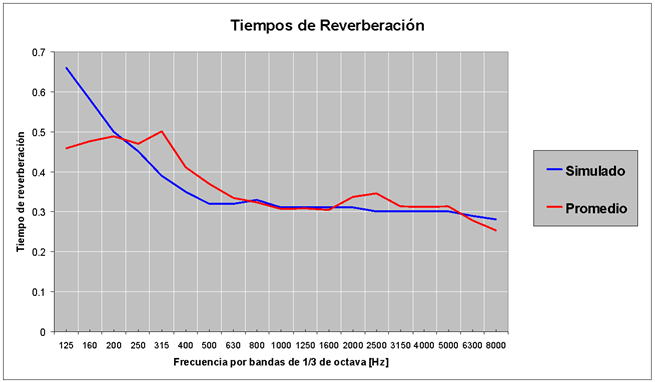
\includegraphics[scale=0.9]{figuras/Tiempo de Reverberacion.png}
        \caption{Comparación de los tiempos de reverberación entre el promedio espacial y la simulación del Hall 4.}
        \label{fig:Tiempo de reverberacion}
    \end{figure}

    \begin{figure}[h]
        \centering
        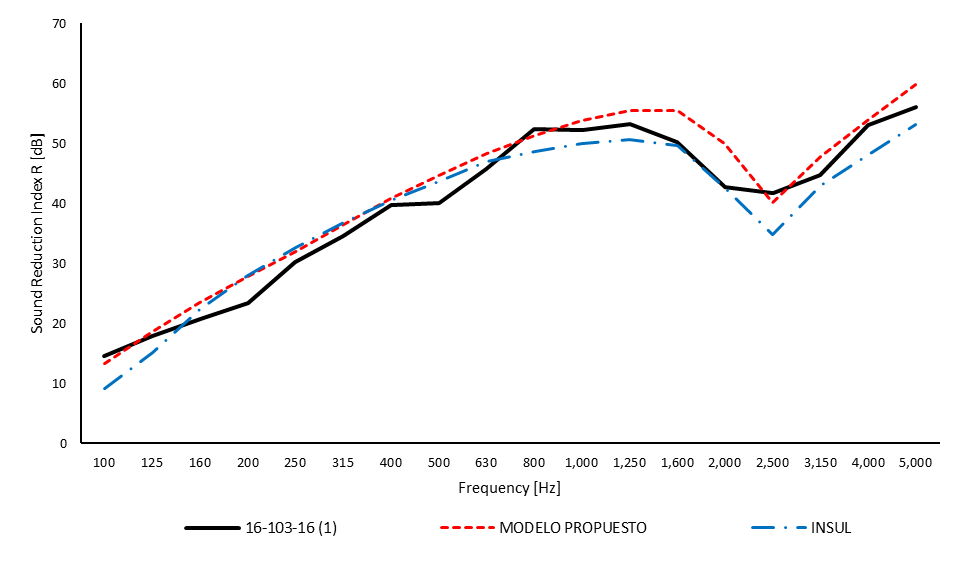
\includegraphics[scale=0.9]{figuras/Comparacion reduccion sonora R.png}
        \caption{Comparativa de los índices de reducción sonora R entre la medición de laboratorio, la predicción del modelo propuesto y el programa INSUL para el caso 1.}
        \label{fig:Comparativa R}
    \end{figure}


\begin{table}
\centering
\begin{tblr}{
  cells = {c},
  hline{1-2,7} = {-}{},
}
\textbf{Material}  & \textbf{Espesor \\\ [mm]} & {\textbf{Densidad}\\\textbf{$[Kg/m^3]$}} & {\textbf{Young}\\\textbf{[GPa]}} & \textbf{Poisson} & {\textbf{Factor de perdidas}\\\textbf{interno}} \\
hormigon  & 50,8; 101,6; 140; 160(x2);& 2100 & 30 & 0,2 & 0,03 \\
Vidrio    & 180; 200; 220; 240              & 2500 & 71 & 0,23& 0,02  \\
placa de yeso & 6,4; 9,5; 12,7; 15.9   & 768  & 2 &  0,23& 0,01  \\
laminado  &  3.2; 6.4                       & 1250 & 3 &  0,15& 0,03  \\
HDF       &  50; 70(x4); 100                &  900 &  3.5& 0,2& 0.005
                                       
\end{tblr}
\caption{Lista de materiales utilizados en la comparativa y sus características físicas.}
\label{Tab:1}
\end{table}

\subsection*{AI 5. \textit{Bibliografía}}
Las referencias a la bibliografía utilizada deberán registrarse en el texto entre corchetes con un número arábigo (Ej [5]). La numeración debe ser consecutiva. En caso de citarse más de una referencia se hará separadas por comas dentro del corchete (Ej [5, 18]) y en caso de necesitar la cita de una sucesión consecutiva de referencias se escribirán separadas por una línea (Ej [5-11]).

La numeración correspondiente a las referencias se podrá incluir al final de la tesis (como se especifica más arriba en la descripción de la Estructura) o bien al final de cada capítulo incluyendo solamente las referencias de ese capítulo. Al utilizar las referencias por capítulo pueden quedar referencias repetidas entre capítulos; en este caso cada capítulo debe ser autocontenido con respecto a las referencias.
